%!TEX root = Bericht.tex
\graphicspath{{graphics/HMI/}{graphics/control_modes/}}
\chapter{Finding a Hardware and Software Solution}
\label{cha:findHardSoftSolution}
References to \cite{kammermann}
\section{Requirements}
\label{sec:requirements}
\textit{Remote Control, Intuitive Control for 6DoF, Livestream, Waypoints}
\section{Existing Solutions}
\label{sec:existingSolutions}
\subsection{Hardware}
\label{sub:hardware}
\textit{RC, Joystick, QGoSphere, 3dMouse, Wii Controller, Smartphones, Tablets, TabletPC}
\subsection{Software}
\textit{QGroundControl, OpenPilot, Qt-Libraries}
\section{Realization}
\label{sec:realization}
\subsection{Compact and Convenient Solution}
\textit{About advantages of TabletPC, 3dMouse, RC}
\subsection{QGroundControl}
\textit{Adaptions in QGroundControl, 3dMouse, Touchscreen, Splines and Trajectory Controller \\ Only how it looks like and how to use. All ``important'' widgets are shown in detail. Implementation of 3dMouse and Touchscreen are not described further.}
\subsection{Mavlink}
\textit{Summary of Protocal, adaptions and use for} \textsc{Skye}




\begin{figure}[h]		
	\small{
		\begin{center}
			\parbox[b]{0.28\textwidth}{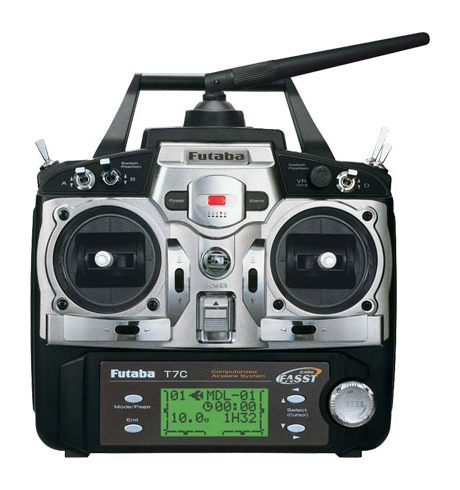
\includegraphics[width=0.28\textwidth]{futaba_7C_radio}
			\begin{center}RC \end{center}}
			\hspace{0.05\textwidth}
			\parbox[b]{0.28\textwidth}{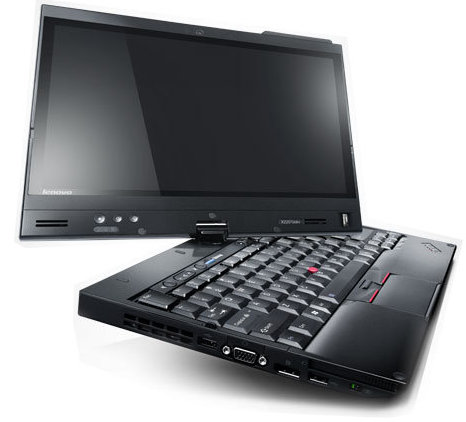
\includegraphics[width=0.28\textwidth]{x220t_hero}
			\begin{center}Tablet \end{center}}
			\hspace{0.05 \textwidth}
			\parbox[b]{0.28\textwidth}{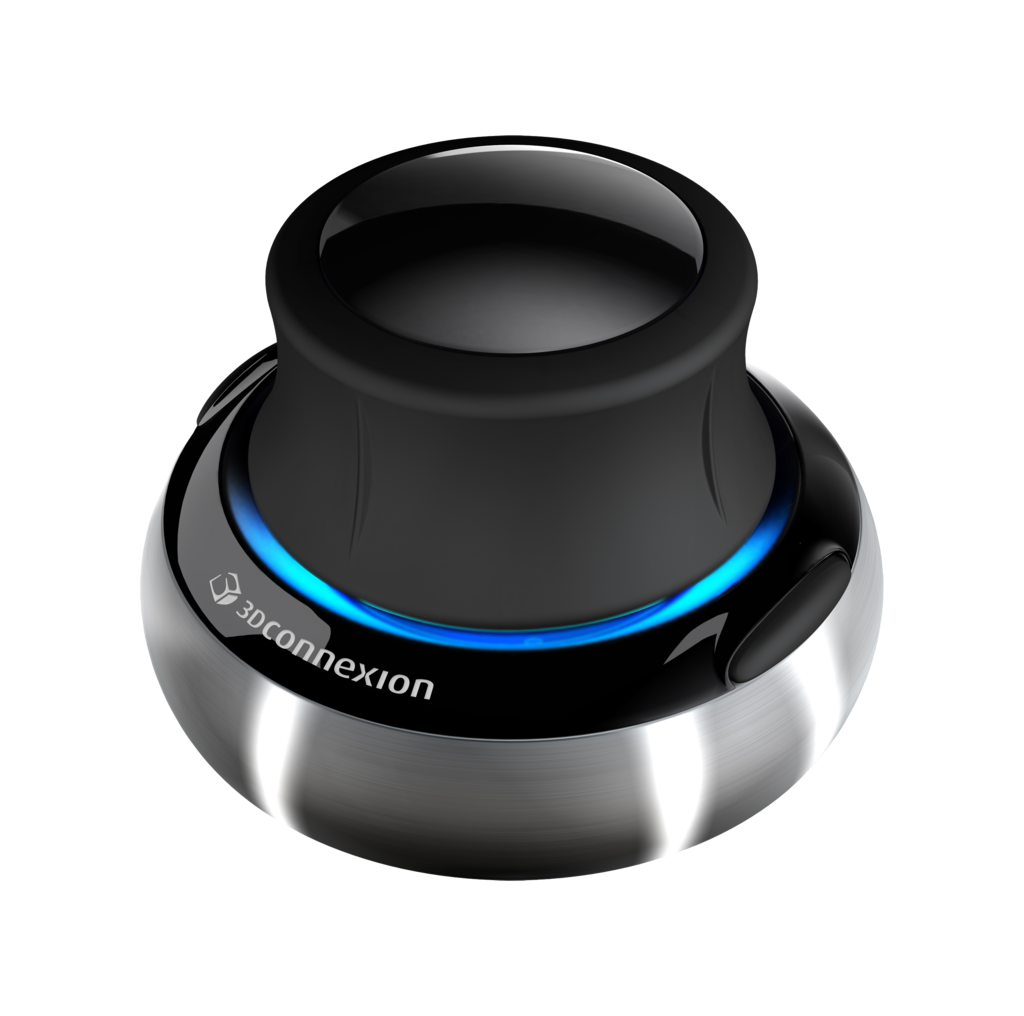
\includegraphics[width=0.28\textwidth]{3dx_productimage}
			\begin{center}3D Mouse \end{center}}			
			\vspace{0.05\textwidth}
			\hspace{0.05\textwidth}			
			\parbox[b]{0.35\textwidth}{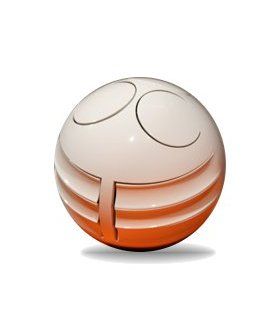
\includegraphics[width=0.35\textwidth]{qgo_sphere_cut}
			\begin{center}Qgo Sphere \end{center}}
			\hspace{0.05\textwidth}
			\parbox[b]{0.35\textwidth}{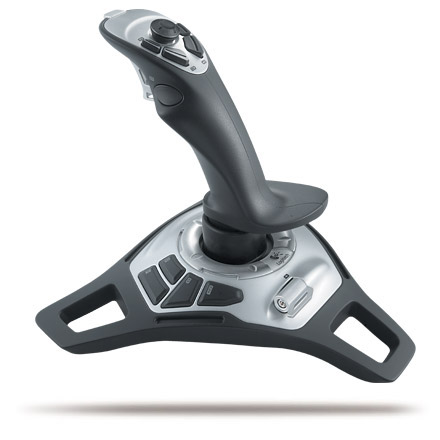
\includegraphics[width=0.35\textwidth]{Logitech-Freedom-Cordless-Joystick}
			\begin{center}Joystick \end{center}}
			\caption[Different devices taken into consideration]{Different devices taken into consideration}
			\label{figure:devices taken into consideration}	
		\end{center}
	}			
	\vspace{4.5mm}
\end{figure}

\begin{table}[H]		% [H] indicates that the table should be right here.
	%\begin{tabularx}{\textwidth}{p{0.125\textwidth}p{0.2\textwidth}|p{0.06\textwidth}p{0.075\textwidth}p{0.08\textwidth}p{0.1\textwidth}p{0.08\textwidth}}	% add p{size_of_colomn} for every new column you'd like to have. If you put a | between the p then there is a vertical line between the columns. 
	\begin{center}
 \begin{tabular}{ll|ccccc}
 \hline
\multicolumn{2}{l|}{Device}	& RC 	& Tablet 	&3D Mouse	&QgoSphere	&Joystick  \\
	\toprule[1.25pt]				%define the line thickness of the top rule
	\multicolumn{2}{l|}{Stand alone}							&\checkmark		&\checkmark		&-			&-			&-\\
	\hline%\midrule
	\multirow{5}{*}{Matching}		&Test Phase					&-				&\checkmark		&-			&-			&-\\
									&Direct Control				&\checkmark		&\checkmark		&\checkmark	&\checkmark	&\checkmark\\
									&Assisted Control			&\checkmark		&\checkmark		&\checkmark	&\checkmark	&\checkmark\\
									&Half Automatic Control		&-				&\checkmark		&-			&-			&- \\
									&Full Automatic Control		&-				&\checkmark		&-			&-			&-\\
	
	\hline%\midrule
	\multicolumn{2}{l|}{Camera View}							&-				&\checkmark		&-			&-			&-\\
	\hline%\midrule
	\multicolumn{2}{l|}{Intuitive}								&quite	&quite	&very&most&quite\\
	\hline%\midrule
	\multicolumn{2}{l|}{Portable}								&most	&quite	&quite&not\footnotemark&quite\\
		
	\bottomrule[1.25pt]
	%\end{tabularx} 
	\end{tabular}
	\caption[Requirements and Expectations for the Hardware]{Requirements and Expectations for the Hardware}
	\label{requirements and expectations for hardware}
	\end{center}
\end{table}
\footnotetext{To detect the sphere's translational movements, a fix-installed infrared sensor is needed.}

\begin{figure}[H] % [H] steht dafür, dass das Bild genau hier im Text sein soll.
	\begin{center}
		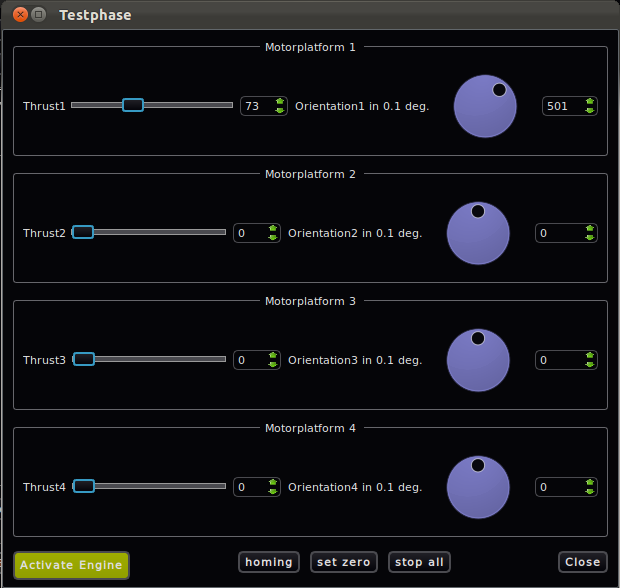
\includegraphics[width=0.7\textwidth]{qgc_test_phase}
		\caption[Test Phase realization]{The \textit{Test Phase} widget allows to adjust each actuation input separately. The input for the four thrusters is set by sliders and the orientation is set by turning the knobs. There is a main button (Activate Engine) to start and stop the motors.}  
		\label{figure:qgc_test_phase}
	\end{center}
\end{figure}

\begin{figure}[H] % [H] steht dafür, dass das Bild genau hier im Text sein soll.
	\begin{center}
		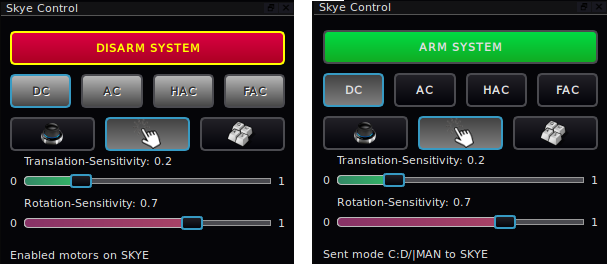
\includegraphics[width=0.6\textwidth]{qgc_skye_control}
		\caption[Main control widget]{On the main control widget, the control mode (Direct Control (DC), Assisted Control (AC), Half Automatic Control (HAC), Full Automatic Control (FAC)) can be set. The colored arm/disarm button is used to (de-)activate the actuators. The input mode (3D Mouse, Touchscreen, Keyboard) can be set by three buttons. The two sliders allow to adjust the input scaling. Indoor flights need usually smaller but more accurate inputs, while outdoors more power is needed.}  
		\label{figure:qgc_skye_control}		
	\end{center}
\end{figure}

\begin{figure}[H] % [H] steht dafür, dass das Bild genau hier im Text sein soll.
	\begin{center}
		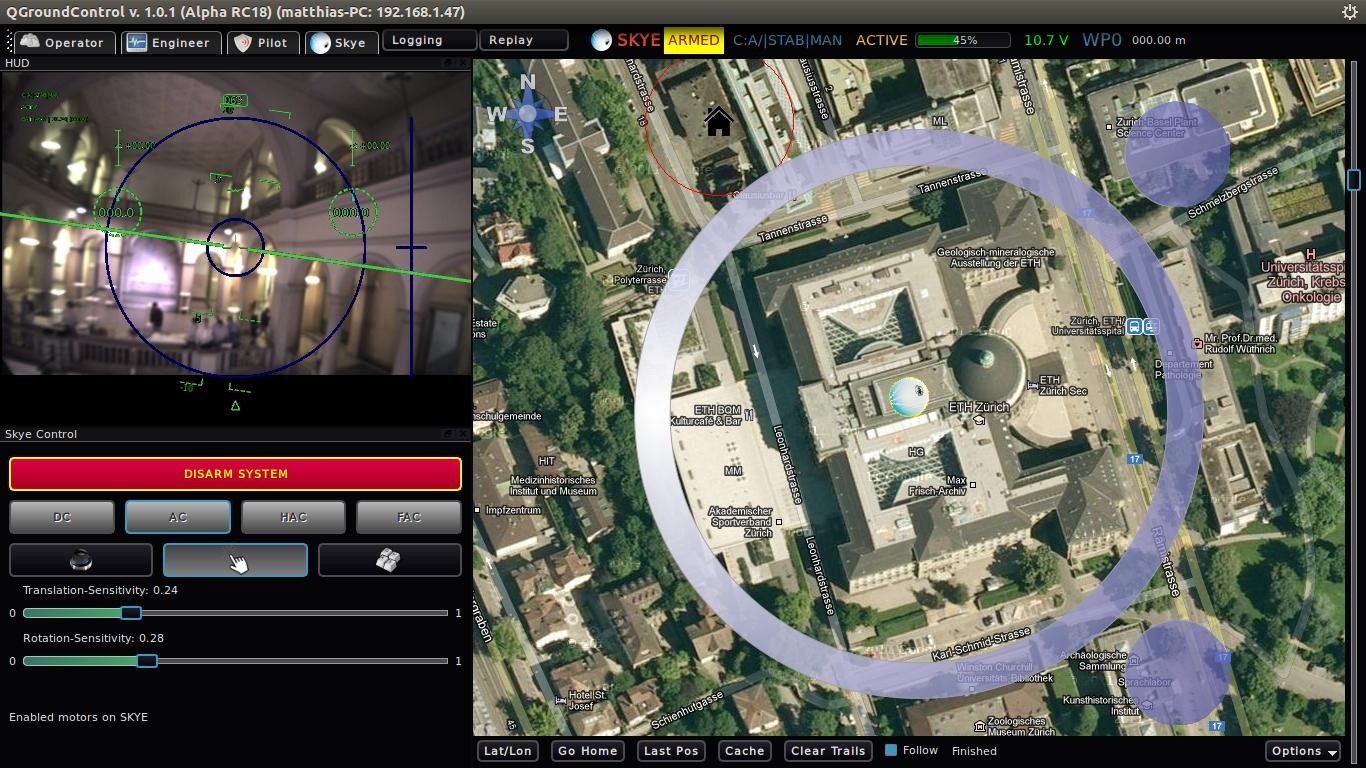
\includegraphics[width=0.8\textwidth]{qgc_manual_control}
		\caption[Manual control view of Graphical User Interface]{The pilots view on the GUI\footnotemark : The HUD shows the video stream and enables rotational touch inputs. The map widget shows the position of \textsc{Skye} and allows to set translational inputs. Note that in a first approach these inputs are always given in the camera frame and not as might expected in inertial frame. Further testing will show which mode is more intuitive. The GUI also includes the main control widget.}  
		\label{figure:qgc_manual_control}		
	\end{center}
\end{figure}
\footnotetext{This screenshot is a reproduced situation of the flight in ETH main building. Obviously, no GPS information were available then.}

\begin{figure}[H] % [H] steht dafür, dass das Bild genau hier im Text sein soll.
	\begin{center}
		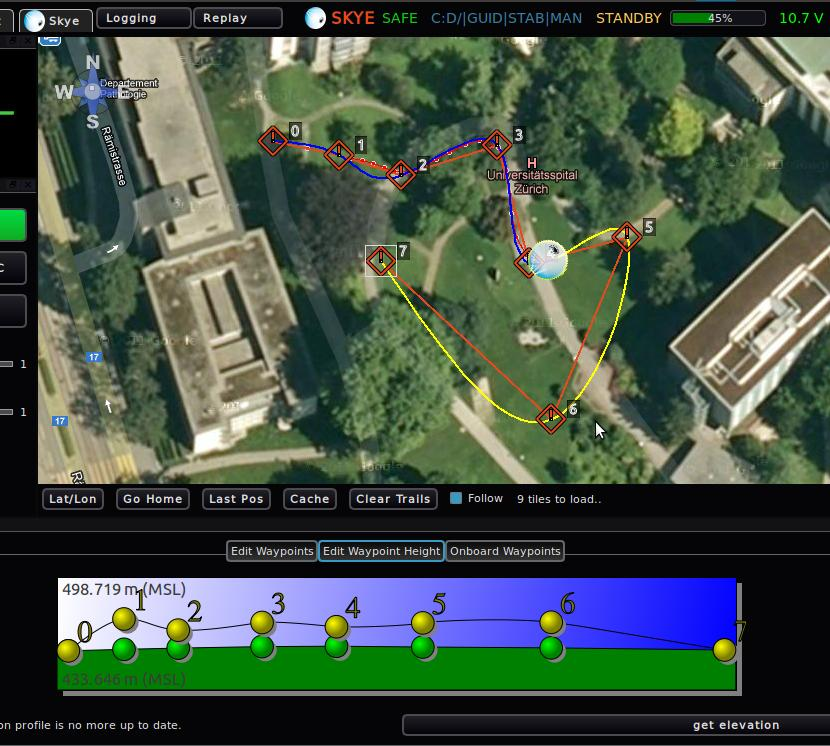
\includegraphics[width=0.8\textwidth]{qgc_automatic_control}
		\caption[Automatic control view of Graphical User Interface]{The user can set waypoints on Google Maps. Spline curves are calculated based on these nodes (yellow line). The part of the path that is already reached is displayed in blue. In the lower part, the height of the waypoints  can be set (yellow points). The actual height of the ground at the waypoints position is also provided by the Google Elevation API\footnotemark (green points and shape). In a further step, the trajectory controlling will be adapted to the real system.}  
		\label{figure:qgc_automatic_control}		
	\end{center}
\end{figure}
\footnotetext{\url{https://developers.google.com/maps/documentation/elevation/}}